\documentclass[11pt]{article}
\usepackage{etex}
\reserveinserts{28}
\usepackage{lastpage}
\usepackage[hmargin=2cm, top=2.7cm, bottom=3.5cm, footskip=0.5cm]{geometry}
\usepackage{url}
\usepackage[maxfloats=50]{morefloats}
\usepackage{parskip}
%\usepackage[citestyle=authoryear-comp,natbib=true]{biblatex}
\usepackage{pdflscape}
\usepackage[absolute]{textpos}
\usepackage{rotating} %for xtable sideways
\usepackage{verbatim}
\usepackage{longtable}
\usepackage{multirow}
\usepackage{lipsum}
%\usepackage[acronym,nomain]{glossaries}
\usepackage{fancyhdr, graphicx, lastpage, ifthen, lscape}
\usepackage[dvipsnames, table]{xcolor}
\usepackage{soul}
\usepackage{booktabs}
\usepackage{setspace}
\usepackage{relsize}
\usepackage{tabularx}
\usepackage{makecell}
\usepackage{threeparttable}
\usepackage{threeparttablex}
\usepackage{hyperref}
\usepackage{float}



\bibliography{/Users/adecamp/Repo/HVTNGitExample/docs/bibliography.bib}


% For knitr
\usepackage{lmodern}
\usepackage{amssymb,amsmath}
\usepackage{ifxetex,ifluatex}
\usepackage{fixltx2e} % provides \textsubscript
\ifnum 0\ifxetex 1\fi\ifluatex 1\fi=0 % if pdftex
  \usepackage[T1]{fontenc}
  \usepackage[utf8]{inputenc}
\else % if luatex or xelatex
  \ifxetex
    \usepackage{mathspec}
    \usepackage{xltxtra,xunicode}
  \else
    \usepackage{fontspec}
  \fi
  \defaultfontfeatures{Mapping=tex-text,Scale=MatchLowercase}
  \newcommand{\euro}{€}
\fi
% use upquote if available, for straight quotes in verbatim environments
\IfFileExists{upquote.sty}{\usepackage{upquote}}{}
% use microtype if available
\IfFileExists{microtype.sty}{%
\usepackage{microtype}
\UseMicrotypeSet[protrusion]{basicmath} % disable protrusion for tt fonts
}{}
\usepackage{color}
\usepackage{fancyvrb}
\newcommand{\VerbBar}{|}
\newcommand{\B}{\rule[-2ex]{0pt}{0pt}} % bottom strut
\newcommand{\VERB}{\Verb[commandchars=\\\{\}]}
\DefineVerbatimEnvironment{Highlighting}{Verbatim}{commandchars=\\\{\}}
% Add ',fontsize=\small' for more characters per line
\usepackage{framed}
\definecolor{shadecolor}{RGB}{248,248,248}
\newenvironment{Shaded}{\begin{snugshade}}{\end{snugshade}}
\newcommand{\AlertTok}[1]{\textcolor[rgb]{0.94,0.16,0.16}{#1}}
\newcommand{\AnnotationTok}[1]{\textcolor[rgb]{0.56,0.35,0.01}{\textbf{\textit{#1}}}}
\newcommand{\AttributeTok}[1]{\textcolor[rgb]{0.77,0.63,0.00}{#1}}
\newcommand{\BaseNTok}[1]{\textcolor[rgb]{0.00,0.00,0.81}{#1}}
\newcommand{\BuiltInTok}[1]{#1}
\newcommand{\CharTok}[1]{\textcolor[rgb]{0.31,0.60,0.02}{#1}}
\newcommand{\CommentTok}[1]{\textcolor[rgb]{0.56,0.35,0.01}{\textit{#1}}}
\newcommand{\CommentVarTok}[1]{\textcolor[rgb]{0.56,0.35,0.01}{\textbf{\textit{#1}}}}
\newcommand{\ConstantTok}[1]{\textcolor[rgb]{0.00,0.00,0.00}{#1}}
\newcommand{\ControlFlowTok}[1]{\textcolor[rgb]{0.13,0.29,0.53}{\textbf{#1}}}
\newcommand{\DataTypeTok}[1]{\textcolor[rgb]{0.13,0.29,0.53}{#1}}
\newcommand{\DecValTok}[1]{\textcolor[rgb]{0.00,0.00,0.81}{#1}}
\newcommand{\DocumentationTok}[1]{\textcolor[rgb]{0.56,0.35,0.01}{\textbf{\textit{#1}}}}
\newcommand{\ErrorTok}[1]{\textcolor[rgb]{0.64,0.00,0.00}{\textbf{#1}}}
\newcommand{\ExtensionTok}[1]{#1}
\newcommand{\FloatTok}[1]{\textcolor[rgb]{0.00,0.00,0.81}{#1}}
\newcommand{\FunctionTok}[1]{\textcolor[rgb]{0.00,0.00,0.00}{#1}}
\newcommand{\ImportTok}[1]{#1}
\newcommand{\InformationTok}[1]{\textcolor[rgb]{0.56,0.35,0.01}{\textbf{\textit{#1}}}}
\newcommand{\KeywordTok}[1]{\textcolor[rgb]{0.13,0.29,0.53}{\textbf{#1}}}
\newcommand{\NormalTok}[1]{#1}
\newcommand{\OperatorTok}[1]{\textcolor[rgb]{0.81,0.36,0.00}{\textbf{#1}}}
\newcommand{\OtherTok}[1]{\textcolor[rgb]{0.56,0.35,0.01}{#1}}
\newcommand{\PreprocessorTok}[1]{\textcolor[rgb]{0.56,0.35,0.01}{\textit{#1}}}
\newcommand{\RegionMarkerTok}[1]{#1}
\newcommand{\SpecialCharTok}[1]{\textcolor[rgb]{0.00,0.00,0.00}{#1}}
\newcommand{\SpecialStringTok}[1]{\textcolor[rgb]{0.31,0.60,0.02}{#1}}
\newcommand{\StringTok}[1]{\textcolor[rgb]{0.31,0.60,0.02}{#1}}
\newcommand{\VariableTok}[1]{\textcolor[rgb]{0.00,0.00,0.00}{#1}}
\newcommand{\VerbatimStringTok}[1]{\textcolor[rgb]{0.31,0.60,0.02}{#1}}
\newcommand{\WarningTok}[1]{\textcolor[rgb]{0.56,0.35,0.01}{\textbf{\textit{#1}}}}
\providecommand{\tightlist}{%
   \setlength{\itemsep}{0pt}\setlength{\parskip}{0pt}}
\makeatletter
\def\maxwidth{\ifdim\Gin@nat@width>\linewidth\linewidth\else\Gin@nat@width\fi}
\def\maxheight{\ifdim\Gin@nat@height>\textheight\textheight\else\Gin@nat@height\fi}
% End For knitr

\renewcommand{\abstractname}{Overview}

% Add unicode checkmark for DataPackageR support. The green checkmark
% that DataPackageR prints to the console during package_build() causes
% an error with latex. This changes the unicode checkmark to a latex one.
\DeclareUnicodeCharacter{2714}{\checkmark}

% Configure hyperref formatting bookmarks and references
\hypersetup{
  colorlinks = true, % color links instead of covering them w/red boxes
  urlcolor   = blue, % color for external hyperlinks
  linkcolor  = cyan, % color of internal links
  citecolor  = gray  % color of citations
}

\newlength{\cslhangindent}
\setlength{\cslhangindent}{1.5em}
\newlength{\csllabelwidth}
\setlength{\csllabelwidth}{3em}
\newenvironment{CSLReferences}[2] % #1 hanging-ident, #2 entry spacing
 {% don't indent paragraphs
  \setlength{\parindent}{0pt}
  % turn on hanging indent if param 1 is 1
  \ifodd #1 \everypar{\setlength{\hangindent}{\cslhangindent}}\ignorespaces\fi
  % set entry spacing
  \ifnum #2 > 0
  \setlength{\parskip}{#2\baselineskip}
  \fi
 }%
 {}
\usepackage{calc}
\newcommand{\CSLBlock}[1]{#1\hfill\break}
\newcommand{\CSLLeftMargin}[1]{\parbox[t]{\csllabelwidth}{#1}}
\newcommand{\CSLRightInline}[1]{\parbox[t]{\linewidth - \csllabelwidth}{#1}\break}
\newcommand{\CSLIndent}[1]{\hspace{\cslhangindent}#1}

%this is to adjust header and footer in landscaped pages
\fancypagestyle{lscape}{%
    \fancyhf{} % clear all header and footer fields
    \fancyhead[R]{\begin{footnotesize}
    \begin{textblock}{1}(0.7,1.5){\color{gray}\rotatebox{90}{Short Title}}\end{textblock}
    \end{footnotesize} }
    \fancyfoot[L]{\begin{footnotesize}
    \begin{textblock}{1}(21,1.75){\color{gray}\rotatebox{90}{Page \thepage{}~of~\pageref{LastPage}}}\end{textblock}
    \end{footnotesize} }
    \fancyfoot[R]{\begin{footnotesize}
%     \begin{textblock}{19.8}[-0.01,{\DynLength}](1.5,23.20){\color{gray}\rotatebox{90}{\Rver}}\end{textblock}
    \begin{textblock}{19.8}(1.5,23.20){\color{gray}\rotatebox{90}{\Rver}}\end{textblock}
    \end{footnotesize} }
    \setlength{\TPHorizModule}{1cm}
    \setlength{\TPVertModule}{1cm}
    \renewcommand{\headrulewidth}{0.0pt}
    \renewcommand{\footrulewidth}{0.0pt}}

%set header and footer for first page
\renewcommand{\headrulewidth}{0.8pt}
\renewcommand{\footrulewidth}{0.8pt}
\fancyhead[L]{\includegraphics[height=0.8cm]{/Library/Frameworks/R.framework/Versions/4.2/Resources/library/VISCtemplates/rmarkdown/templates/visc_report/resources/SCHARP_logo.png}}
\fancyhead[C]{\includegraphics[height=0.8cm]{/Library/Frameworks/R.framework/Versions/4.2/Resources/library/VISCtemplates/rmarkdown/templates/visc_report/resources/VISC_logo.jpg}}
\fancyhead[R]{\includegraphics[height=0.8cm]{/Library/Frameworks/R.framework/Versions/4.2/Resources/library/VISCtemplates/rmarkdown/templates/visc_report/resources/FredHutch_logo.png}}
\fancyfoot[C]{Page \thepage{}~of~\pageref{LastPage}}
\setlength{\headheight}{27pt}

%decrease margins for landscape pages
\newenvironment{changemargin}[2]{%
\begin{list}{}{%
\setlength{\topsep}{0pt}%
\setlength{\leftmargin}{#1}%
\setlength{\rightmargin}{#2}%
%\setlength{\listparindent}{\parindent}%
%\setlength{\itemindent}{\parindent}%
\setlength{\parsep}{\parskip}%
}%
\item[]}{\end{list}}

% being able to set emphasis for entire table row
\newcommand\setrow[1]{\gdef\rowmac{#1}#1\ignorespaces}
\newcommand\clearrow{\global\let\rowmac\relax}
\clearrow

%page settings
\setlength{\footskip}{56pt}
\pagestyle{fancy}
\setlength{\parindent}{0pt}
%\makeglossaries
\begin{document}
\sloppy

%get current date into insertdate
\makeatletter
\let\insertdate\@date
\makeatother

% workaround to use landscape environment with pandoc
\newcommand{\blandscape}{\begin{landscape}}
\newcommand{\elandscape}{\end{landscape}}

%begin To and From Section
\makeatletter
\newcommand\tabfill[1]{%
  \dimen@\linewidth
  \advance\dimen@\@totalleftmargin
  \advance\dimen@-\dimen\@curtab
  \parbox[t]\dimen@{%
    \leftskip=2em\hspace*{-2em}#1\ifhmode\strut\fi}%
}
\makeatother

\vspace{0.1cm}
\begin{flushleft}
\begin{tabbing}
this line is to\= set up the tab stop \kill
{\bf Date:} \> \insertdate\\
{\bf To:} \>  \tabfill{FirstNameA LastNameA, FirstNameB LastNameB, FirstNameC LastNameC, FirstNameD LastNameD, FirstNameE LastNameE, FirstNameF LastNameF}\\
{\bf From:} \> \tabfill{FirstNameA LastNameA, FirstNameB LastNameB}\\
{\bf RE:} \> \tabfill{Title of Your Submission}\\
{\bf cc:} \> \tabfill{FirstNameA LastNameA, FirstNameB LastNameB, FirstNameC LastNameC, FirstNameD LastNameD, FirstNameE LastNameE}\\
{\bf Contact:} \> \tabfill{FirstNameA LastNameA, \href{mailto:foo@bar.com}{\nolinkurl{foo@bar.com}}  }\\
\end{tabbing}
\end{flushleft}

\hrule

\vspace{2cm}

%begin contents section
\tableofcontents

%change color of header and footer text to gray
\makeatletter
\patchcmd{\@fancyhead}{\rlap}{\color{gray}\rlap}{}{}
\patchcmd{\headrule}{\hrule}{\color{gray}\hrule}{}{}
\patchcmd{\@fancyfoot}{\rlap}{\color{gray}\rlap}{}{}
\patchcmd{\footrule}{\hrule}{\color{gray}\hrule}{}{}
\makeatother


\begin{abstract}
A short summary about your report.
\end{abstract}

\listoffigures

\listoftables

\newpage
\fancyhead[R]{\em Short Title}
\fancyhead[C]{}
\fancyhead[L]{\em VISC Report}
%\printglossaries

\clearpage

\hypertarget{summary-of-main-results}{%
\section{Summary of Main Results}\label{summary-of-main-results}}

Summarize the main highlights from the Results section.
This can be in bullet format.
Any significant results mentioned should include p-values and references to
appropriate figures and tables.
There should be no information in the Summary section that is not contained in
the Results section (see \ref{results}).

\hypertarget{background}{%
\section{Background}\label{background}}

This document should contain the study background section for HVTNGitExample.

Write project background here. Don't use headers.

This report presents data {[}blinded/unblinded{]} to treatment arm,
as of {[}enter date of data file creation{]}.

Samples were collected at:
{[}list study time points and corresponding relationship to vaccination,
e.g., week 0 (1st vaccination),
week 6 (2 weeks post-2nd vaccination),
week 10 (2 weeks post-3rd vaccination,
and week 26 (2 weeks post-4th (final) vaccination)){]}
for {[}\# groups; list vaccine doses or group descriptions{]}
(reference test: Huang and Gottardo (2013)).

\begin{table}[!h]

\caption{\label{tab:study-schema}HVTNGitExample study schema.}
\centering
\begin{tabular}[t]{lrll}
\toprule
Group & Sample Size & Week 10 & Week 20\\
\midrule
Group A & 10 & Dose A & Dose A\\
Group B & 10 & Dose B & Dose B\\
\bottomrule
\end{tabular}
\end{table}

\hypertarget{report-amendments}{%
\subsection{Report Amendments}\label{report-amendments}}

If previous reports were provided, note if this report supplements or supersedes
the previous reports.
For example, ``the previous PT report (distributed on DDMonthYYYY) presented
peak data. This report summarizes additional durability data.''

If this is an updated report, also briefly describe additional data included
and/or analysis done since the previous report (e.g., additional visits,
participants (include pubIDs), antigens, comparisons, new/changed tables, figures).

\hypertarget{objectives}{%
\section{Objectives}\label{objectives}}

List primary and secondary (if applicable) objectives.
Objectives can be found on ATLAS, in the study protocol, or in the SAP.

\hypertarget{biological-endpoints}{%
\section{Biological Endpoints}\label{biological-endpoints}}

Describe the lab measures of interest and the antigens/isolates tested.
The biological endpoints may be in the SAP, or you may need to contact the lab
for details. This may be done at the lab review stage.
Make sure to this section is written in the past tense.

\hypertarget{lab-methods}{%
\section{Lab Methods}\label{lab-methods}}

Describe the lab methods.
The lab methods section is written by the lab.
Use template language prior to lab review, and then the lab can make changes to
this section during their review.

\hypertarget{statistical-methods}{%
\section{Statistical Methods}\label{statistical-methods}}

\hypertarget{statistical-endpoints}{%
\subsection{Statistical Endpoints}\label{statistical-endpoints}}

Describe the statistical measures of interest (response, response magnitude, etc.)
including response call methodology and truncation, if applicable.

\hypertarget{graphical-analysis}{%
\subsection{Graphical Analysis}\label{graphical-analysis}}

Update the following section as appropriate for your data.

Response rates were plotted, with accompanying Wilson score confidence intervals,
for each group, antigen, and study time point.
Distributions of response magnitude were plotted on the log scale for each
group, antigen, and study time point with box plots superimposed on the
distribution of responders.
The mid-line of the box denotes the median and the ends of the box denote
the \(25^{th}\) and \(75^{th}\) percentiles.
The whiskers denote the most extreme data points that were no more than 1.5
times the interquartile range (i.e., height of the box).
To show response trend over time, line plots of response magnitude were plotted
on the log scale by study group and antigen across time points.

\hypertarget{statistical-tests}{%
\subsection{Statistical Tests}\label{statistical-tests}}

Update the following section as appropriate for your data. If available, use
language from the statistical analysis plan. Ensure that this section includes
all statistical methodology used in the report.

To assess if two groups have different response rates, pairwise group
comparisons were conducted using Fisher's exact test for each time point and
antigen.

For comparisons across time, McNemar's test were used to account for paired data.
Response magnitude comparisons between experimental groups were compared using
the Wilcoxon rank-sum test {[}among responders only{]}.
Response magnitude comparisons between time points were performed using the
Wilcoxon signed-rank test to account for paired data.

\hypertarget{participant-cohort}{%
\section{Participant Cohort}\label{participant-cohort}}

The study enrolled {[}describe the total number enrolled to date and, if unblinded,
the number in each treatment arm{]}.
Include a table with data availability by key variables and red highlights for
counts that are less than expected.
Refer to the table and comment on reasons for missing data if known.

\hypertarget{results}{%
\section{Results}\label{results}}

The results section addresses how each endpoint supports the main objectives.
Include summary statistics and significant results as applicable,
including p-values and table and figure references.
The results section should provide supporting evidence for all statements made
in the summary section.

\hypertarget{section-1}{%
\subsection{Section 1}\label{section-1}}

Consider breaking up the results section by objective or by statistical endpoint.

\hypertarget{section-2}{%
\subsection{Section 2}\label{section-2}}

Make sure to include p-values and references to relevant tables and figures.
See Figure \ref{fig:example-plot} and Table \ref{tab:example-tab}.

\clearpage

\hypertarget{figures-and-tables}{%
\section{Figures and Tables}\label{figures-and-tables}}

\begin{figure}[H]

{\centering 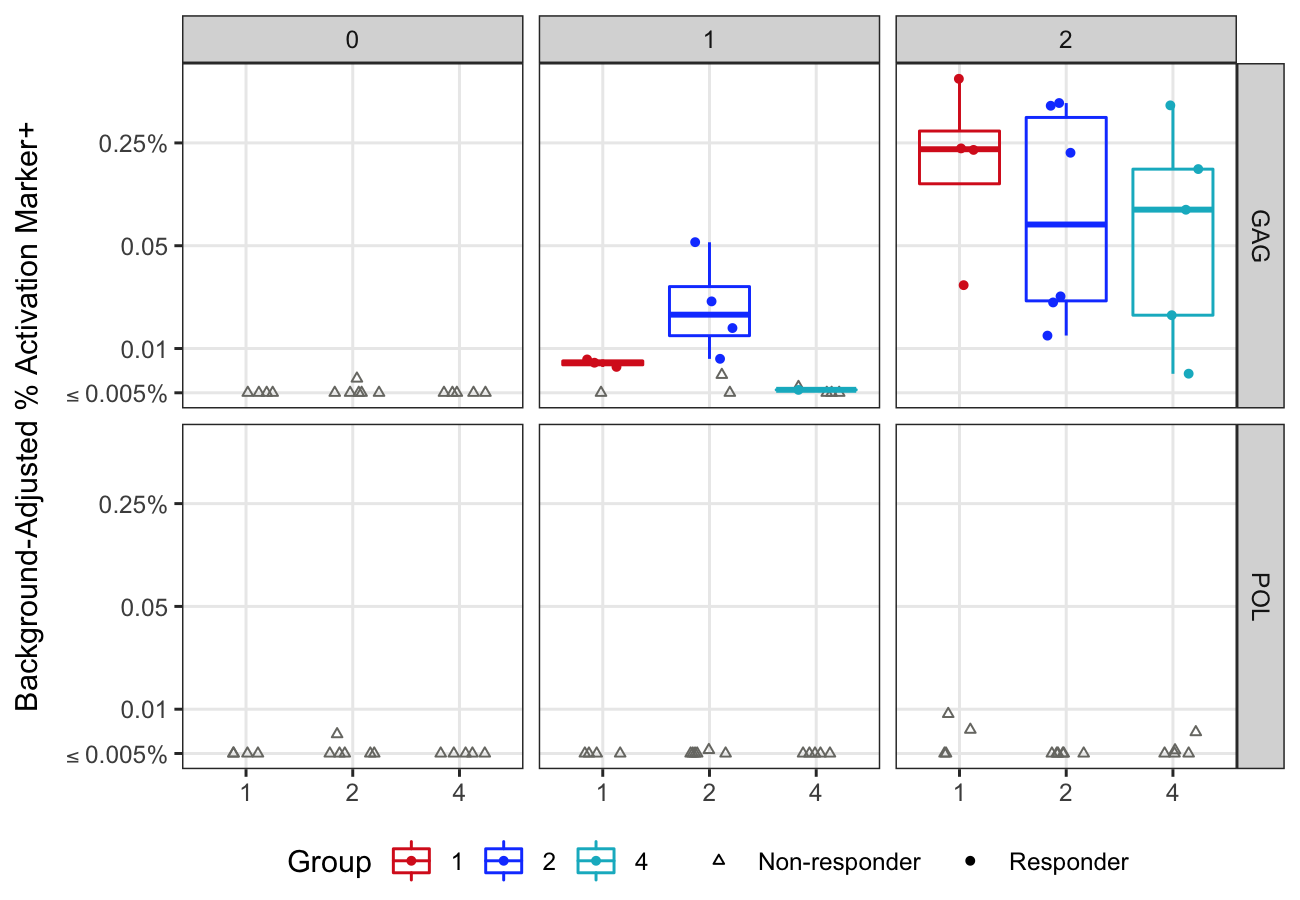
\includegraphics[width=1\linewidth,]{HVTN_Workshop_Example_files/figure-latex/example-plot-1} 

}

\caption[Shorter caption for List of Figures.]{Longer caption that shows under the figure. Explain everything needed to understand the figure here.}\label{fig:example-plot}
\end{figure}

\clearpage

\begin{table}[!h]

\caption[Short caption to show in List of Tables.]{\label{tab:example-tab}Long caption to show above table. Explain everything needed to understand the table here.}
\centering
\resizebox{\linewidth}{!}{
\fontsize{8}{10}\selectfont
\begin{threeparttable}
\begin{tabular}[t]{lrlllll}
\toprule
Stim & Visit & Comparison & SampleSizes & Median (Range) & Mean (SD) & MagnitudeTest\\
\midrule
 &  & 1 > 2 & 4 vs. 6 & 0.000 [0.000, 0.002] vs. 0.000 [0.000, 0.006] & 0.001 (0.001) vs. 0.001 (0.003) & 0.667\\
\cmidrule{3-7}
 &  & 1 > 4 & 4 vs. 5 & 0.000 [0.000, 0.002] vs. 0.000 [0.000, 0.000] & 0.001 (0.001) vs. 0.000 (0.000) & 0.444\\
\cmidrule{3-7}
 & \multirow{-3}{*}{\raggedleft\arraybackslash 0} & 2 > 4 & 6 vs. 5 & 0.000 [0.000, 0.006] vs. 0.000 [0.000, 0.000] & 0.001 (0.003) vs. 0.000 (0.000) & 0.273\\
\cmidrule{2-7}
 &  & 1 > 2 & 4 vs. 6 & 0.008 [0.004, 0.008] vs. 0.011 [0.003, 0.053] & 0.007 (0.002) vs. 0.018 (0.018) & 0.871\\
\cmidrule{3-7}
 &  & 1 > 4 & 4 vs. 5 & 0.008 [0.004, 0.008] vs. 0.002 [-0.005, 0.005] & 0.007 (0.002) vs. 0.002 (0.004) & \cellcolor{yellow}{0.032}\\
\cmidrule{3-7}
 & \multirow{-3}{*}{\raggedleft\arraybackslash 1} & 2 > 4 & 6 vs. 5 & 0.011 [0.003, 0.053] vs. 0.002 [-0.005, 0.005] & 0.018 (0.018) vs. 0.002 (0.004) & \cellcolor{yellow}{0.009}\\
\cmidrule{2-7}
 &  & 1 > 2 & 4 vs. 6 & 0.226 [0.027, 0.683] vs. 0.119 [0.012, 0.466] & 0.291 (0.278) vs. 0.197 (0.215) & 0.176\\
\cmidrule{3-7}
 &  & 1 > 4 & 4 vs. 5 & 0.226 [0.027, 0.683] vs. 0.088 [0.007, 0.450] & 0.291 (0.278) vs. 0.145 (0.182) & 0.143\\
\cmidrule{3-7}
\multirow{-9}{*}{\raggedright\arraybackslash GAG} & \multirow{-3}{*}{\raggedleft\arraybackslash 2} & 2 > 4 & 6 vs. 5 & 0.119 [0.012, 0.466] vs. 0.088 [0.007, 0.450] & 0.197 (0.215) vs. 0.145 (0.182) & 0.331\\
\cmidrule{1-7}
 &  & 1 > 2 & 4 vs. 6 & 0.000 [0.000, 0.003] vs. 0.000 [0.000, 0.007] & 0.001 (0.002) vs. 0.001 (0.003) & 0.667\\
\cmidrule{3-7}
 &  & 1 > 4 & 4 vs. 5 & 0.000 [0.000, 0.003] vs. 0.000 [0.000, 0.003] & 0.001 (0.002) vs. 0.001 (0.002) & 0.722\\
\cmidrule{3-7}
 & \multirow{-3}{*}{\raggedleft\arraybackslash 0} & 2 > 4 & 6 vs. 5 & 0.000 [0.000, 0.007] vs. 0.000 [0.000, 0.003] & 0.001 (0.003) vs. 0.001 (0.002) & 0.697\\
\cmidrule{2-7}
 &  & 1 > 2 & 4 vs. 6 & 0.002 [0.000, 0.005] vs. 0.000 [0.000, 0.005] & 0.002 (0.002) vs. 0.001 (0.002) & 0.452\\
\cmidrule{3-7}
 &  & 1 > 4 & 4 vs. 5 & 0.002 [0.000, 0.005] vs. 0.000 [-0.005, 0.001] & 0.002 (0.002) vs. -0.001 (0.002) & 0.127\\
\cmidrule{3-7}
 & \multirow{-3}{*}{\raggedleft\arraybackslash 1} & 2 > 4 & 6 vs. 5 & 0.000 [0.000, 0.005] vs. 0.000 [-0.005, 0.001] & 0.001 (0.002) vs. -0.001 (0.002) & 0.132\\
\cmidrule{2-7}
 &  & 1 > 2 & 4 vs. 6 & 0.004 [-0.001, 0.009] vs. 0.001 [-0.016, 0.004] & 0.004 (0.005) vs. -0.001 (0.007) & 0.381\\
\cmidrule{3-7}
 &  & 1 > 4 & 4 vs. 5 & 0.004 [-0.001, 0.009] vs. 0.001 [-0.002, 0.007] & 0.004 (0.005) vs. 0.002 (0.004) & 0.365\\
\cmidrule{3-7}
\multirow{-9}{*}{\raggedright\arraybackslash POL} & \multirow{-3}{*}{\raggedleft\arraybackslash 2} & 2 > 4 & 6 vs. 5 & 0.001 [-0.016, 0.004] vs. 0.001 [-0.002, 0.007] & -0.001 (0.007) vs. 0.002 (0.004) & 0.686\\
\bottomrule
\end{tabular}
\begin{tablenotes}
\item \textit{Note: } 
\item SD: standard deviation.
\end{tablenotes}
\end{threeparttable}}
\end{table}

\clearpage

\begin{table}

\caption{\label{tab:Software-Session-Information}Reproducibility software session information}
\centering
\fontsize{10}{12}\selectfont
\begin{tabular}[t]{ll}
\toprule
name & value\\
\midrule
version & R version 4.2.1 (2022-06-23)\\
os & macOS Big Sur ... 10.16\\
system & x86\_64, darwin17.0\\
ui & X11\\
language & (EN)\\
collate & en\_US.UTF-8\\
ctype & en\_US.UTF-8\\
tz & America/Los\_Angeles\\
date & 2022-10-25\\
pandoc & 2.19.2 @ /Applications/RStudio.app/Contents/MacOS/quarto/bin/tools/ (via rmarkdown)\\
repo & git@github.com:adecamp/HVTNGitExample.git\\
file name & HVTN\_Workshop\_Example.Rmd\\
location & HVTN\_Workshop\_Example\\
user & adecamp\\
\bottomrule
\end{tabular}
\end{table}

\begin{table}

\caption{\label{tab:Software-Package-Version-Information}Reproducibility software package version information}
\centering
\fontsize{10}{12}\selectfont
\begin{tabular}[t]{llll}
\toprule
package & version & date & source\\
\midrule
conflicted & 1.1.0 & 2021-11-26 & CRAN (R 4.2.0)\\
dplyr & 1.0.9 & 2022-04-28 & CRAN (R 4.2.0)\\
forcats & 0.5.1 & 2021-01-27 & CRAN (R 4.2.0)\\
ggplot2 & 3.3.6 & 2022-05-03 & CRAN (R 4.2.0)\\
here & 1.0.1 & 2020-12-13 & CRAN (R 4.2.0)\\
kableExtra & 1.3.4 & 2021-02-20 & CRAN (R 4.2.0)\\
knitr & 1.40 & 2022-08-24 & CRAN (R 4.2.0)\\
purrr & 0.3.5 & 2022-10-06 & CRAN (R 4.2.0)\\
readr & 2.1.2 & 2022-01-30 & CRAN (R 4.2.0)\\
rmarkdown & 2.17 & 2022-10-07 & CRAN (R 4.2.0)\\
stringr & 1.4.1 & 2022-08-20 & CRAN (R 4.2.0)\\
tibble & 3.1.7 & 2022-05-03 & CRAN (R 4.2.0)\\
tidyr & 1.2.0 & 2022-02-01 & CRAN (R 4.2.0)\\
tidyverse & 1.3.1 & 2021-04-15 & CRAN (R 4.2.0)\\
VISCfunctions & 1.2.2 & 2022-06-29 & Github (FredHutch/VISCfunctions@28be2826df1c09cf2cac919ae2db82e05dde8dd9)\\
VISCtemplates & 1.1.0 & 2022-10-25 & Github (FredHutch/VISCtemplates@5c2da0e37c313fc59a3e01caa44777843b810c12)\\
\bottomrule
\end{tabular}
\end{table}

\clearpage

\hypertarget{references}{%
\section*{References}\label{references}}
\addcontentsline{toc}{section}{References}

\hypertarget{refs}{}
\begin{CSLReferences}{1}{0}
\leavevmode\vadjust pre{\hypertarget{ref-Huang:2013fl}{}}%
Huang, Yunda, and Raphaël Gottardo. 2013. {``Comparability and Reproducibility of Biomedical Data.''} \emph{Briefings in Bioinformatics} 14 (4): 391--401.

\end{CSLReferences}
\label{LastPageOfBackMatter}~
\end{document}
